\documentclass{article}\usepackage[]{graphicx}\usepackage[]{xcolor}
% maxwidth is the original width if it is less than linewidth
% otherwise use linewidth (to make sure the graphics do not exceed the margin)
\makeatletter
\def\maxwidth{ %
  \ifdim\Gin@nat@width>\linewidth
    \linewidth
  \else
    \Gin@nat@width
  \fi
}
\makeatother

\definecolor{fgcolor}{rgb}{0.345, 0.345, 0.345}
\newcommand{\hlnum}[1]{\textcolor[rgb]{0.686,0.059,0.569}{#1}}%
\newcommand{\hlstr}[1]{\textcolor[rgb]{0.192,0.494,0.8}{#1}}%
\newcommand{\hlcom}[1]{\textcolor[rgb]{0.678,0.584,0.686}{\textit{#1}}}%
\newcommand{\hlopt}[1]{\textcolor[rgb]{0,0,0}{#1}}%
\newcommand{\hlstd}[1]{\textcolor[rgb]{0.345,0.345,0.345}{#1}}%
\newcommand{\hlkwa}[1]{\textcolor[rgb]{0.161,0.373,0.58}{\textbf{#1}}}%
\newcommand{\hlkwb}[1]{\textcolor[rgb]{0.69,0.353,0.396}{#1}}%
\newcommand{\hlkwc}[1]{\textcolor[rgb]{0.333,0.667,0.333}{#1}}%
\newcommand{\hlkwd}[1]{\textcolor[rgb]{0.737,0.353,0.396}{\textbf{#1}}}%
\let\hlipl\hlkwb

\usepackage{framed}
\makeatletter
\newenvironment{kframe}{%
 \def\at@end@of@kframe{}%
 \ifinner\ifhmode%
  \def\at@end@of@kframe{\end{minipage}}%
  \begin{minipage}{\columnwidth}%
 \fi\fi%
 \def\FrameCommand##1{\hskip\@totalleftmargin \hskip-\fboxsep
 \colorbox{shadecolor}{##1}\hskip-\fboxsep
     % There is no \\@totalrightmargin, so:
     \hskip-\linewidth \hskip-\@totalleftmargin \hskip\columnwidth}%
 \MakeFramed {\advance\hsize-\width
   \@totalleftmargin\z@ \linewidth\hsize
   \@setminipage}}%
 {\par\unskip\endMakeFramed%
 \at@end@of@kframe}
\makeatother

\definecolor{shadecolor}{rgb}{.97, .97, .97}
\definecolor{messagecolor}{rgb}{0, 0, 0}
\definecolor{warningcolor}{rgb}{1, 0, 1}
\definecolor{errorcolor}{rgb}{1, 0, 0}
\newenvironment{knitrout}{}{} % an empty environment to be redefined in TeX

\usepackage{alltt}
\usepackage[utf8]{inputenc}
\usepackage{amsfonts}
\usepackage{tgpagella}
\usepackage{graphicx} % Required for inserting images
\usepackage{polski}
\renewcommand*{\figurename}{Rysunek}
\usepackage{nicefrac, xfrac}
\usepackage[margin=1in]{geometry}
\usepackage{hyperref}
\usepackage{xcolor}
\usepackage{amssymb}
\usepackage[bottom]{footmisc}
\usepackage{float}
\IfFileExists{upquote.sty}{\usepackage{upquote}}{}
\begin{document}



\section{Odsetek naprawianych marek pojazdów}
%Odsetek naprawianych marek pojazdów.

Przeprowadzono analizę, aby sprawdzić jakich marek pojazdy najczęściej pojawiają się w warsztacie do naprawy. 



Można przedstawić procentowy udział marek pojazdów klientów salonu, zaczynając od najczęściej się pojawiającej:

\begin{verbatim}
1. Volkswagen: 14.22%
2. Opel: 11.61%
3. Ford: 8.77%
4. Renault: 6.16%
5. Audi: 6.16%
6. Hyundai: 4.98%
7. Skoda: 4.98%
8. Fiat: 4.74%
9. Bajaj: 4.27%
10. Mercedes-Benz: 3.79%
11. Citroen: 3.08%
12. SEAT: 3.08%
13. BMW: 3.08%
14. Honda: 2.61%
15. Kia: 2.37%
16. Suzuki: 2.37%
17. Nissan: 2.13%
18. Peugeot: 2.13%
19. Mazda: 1.9%
20. Yamaha: 1.66%
21. Hero: 1.42%
22. Toyota: 1.42%
23. TVS: 1.42%
24. Volvo: 1.18%
25. Mitsubishi: 0.95%
26. Dacia: 0.71%
27. Porsche: 0.71%
28. Royal: 0.47%
29. MINI: 0.24%
30. Dodge: 0.24%
31. Vespa: 0.24%
32. Microcar: 0.24%
33. Jeep: 0.24%
34. Chevrolet: 0.24%
35. Mahindra: 0.24%
36. Jaguar: 0.24%
37. SsangYong: 0.24%
\end{verbatim}

Jak widać, najpopularniejsze są pojazdy marki Volkswagen. Pojazdy tej marki stanowią 14.22\% wszystkich. \\

Najmniej popularne są marki Dodge, Vespa, Microcar, Jeep, Chevrolet, Mahindra, Jaguar, SsangYong i MINI. Każdą z nich reprezentowało 0.24\% pojazdów, które się pojawiły w warsztacie.

Sprawdzono także, jak prezentowałyby się rozkład marek, gdyby brano pod uwagę jedynie samochody



Można przedstawić ranking marek, zaczynając od najczęściej się pojawiającej:

\begin{verbatim}
1. Volkswagen: 16.13%
2. Opel: 13.17%
3. Ford: 9.95%
4. Audi: 6.99%
5. Renault: 6.99%
6. Hyundai: 5.65%
7. Skoda: 5.65%
8. Fiat: 5.38%
9. Mercedes-Benz: 4.3%
10. BMW: 3.49%
11. SEAT: 3.49%
12. Citroen: 3.49%
13. Kia: 2.69%
14. Nissan: 2.42%
15. Peugeot: 2.42%
16. Mazda: 2.15%
17. Suzuki: 1.88%
18. Toyota: 1.61%
19. Volvo: 1.34%
20. Mitsubishi: 1.08%
21. Dacia: 0.81%
22. Porsche: 0.81%
23. Honda: 0.81%
24. MINI: 0.27%
25. Jeep: 0.27%
26. SsangYong: 0.27%
27. Microcar: 0.27%
28. Jaguar: 0.27%
29. Dodge: 0.27%
30. Chevrolet: 0.27%
\end{verbatim}

Wśród aut prym wiedzie Volkswagen, reprezentując  16.13\% naprawianych samochodów. \\

Najmniej było samochodów marek Jeep, SsangYong, Microcar, Jaguar, Dodge, Chevrolet i MINI. Było ich 0.27\% dla każdej. \\

{\color{red} Coś o tym, czy się zgadza z pojazdami}

Pozostały do sprawdzenia motory.



Udział procentowy poszczególnych marek wśród nich prezentuje się następująco:

\begin{verbatim}
1. Bajaj: 36%
2. Honda: 16%
3. Yamaha: 14%
4. TVS: 12%
5. Hero: 12%
6. Suzuki: 6%
7. Royal: 4%
8. Vespa: 2%
9. Mahindra: 2%
\end{verbatim}

Wśród nich najczęściej naprawiano motory marki Bajaj. Pojazdy tej marki stanowią 36.00\% wszystkich. \\

Najmniej popularnymi motorami są z kolei modele marek Mahindra i Vespa. W warsztacie było zaledwie 2.00\% motorów każdej z wymienionych marek.

{\color{red} Coś o tym, czy się zgadza z pojazdami}

\section{Analiza bilansu}

\subsection{Analiza wydatków na zakup pojazdów}

\begin{knitrout}
\definecolor{shadecolor}{rgb}{0.969, 0.969, 0.969}\color{fgcolor}
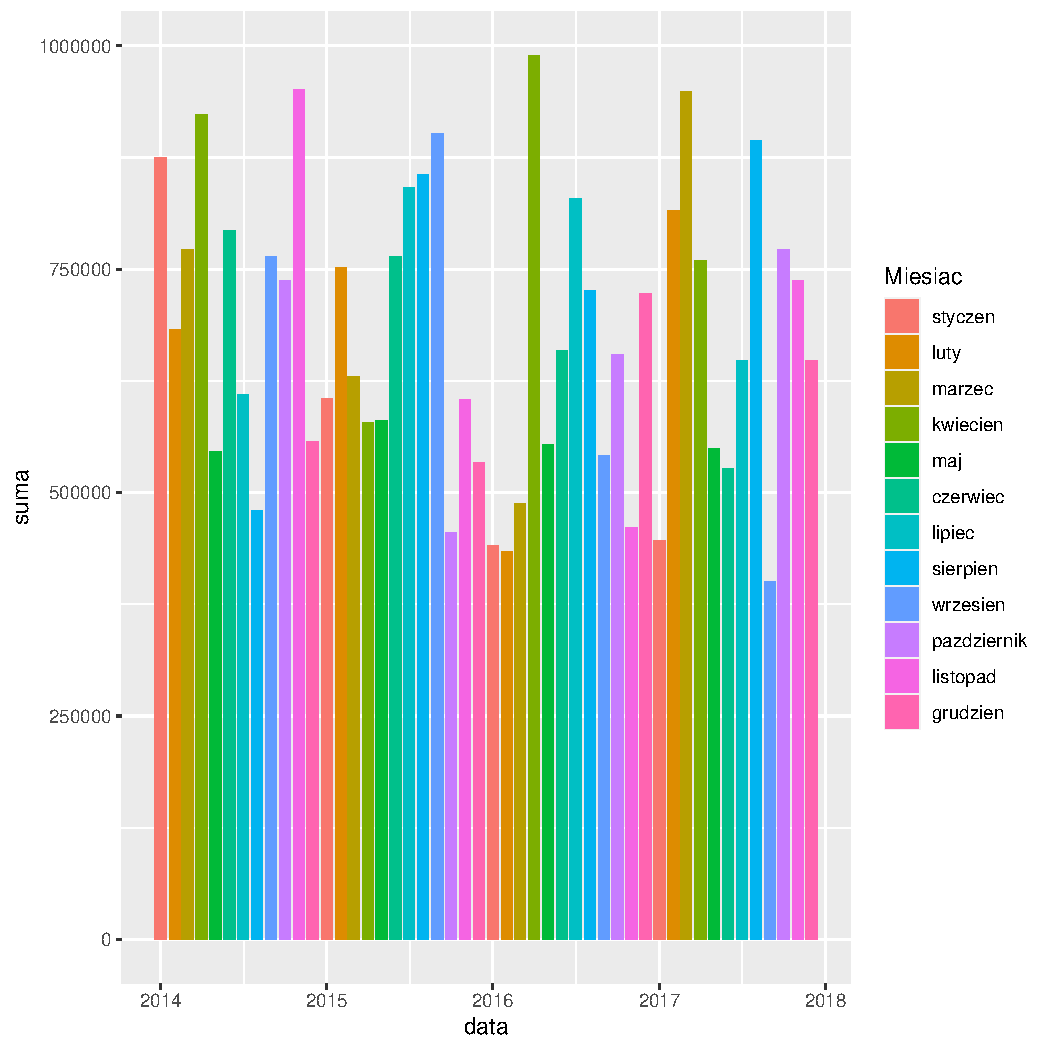
\includegraphics[width=\maxwidth]{figure/unnamed-chunk-5-1} 
\end{knitrout}


\subsection{Analiza wydatków na zakup części}

\begin{knitrout}
\definecolor{shadecolor}{rgb}{0.969, 0.969, 0.969}\color{fgcolor}
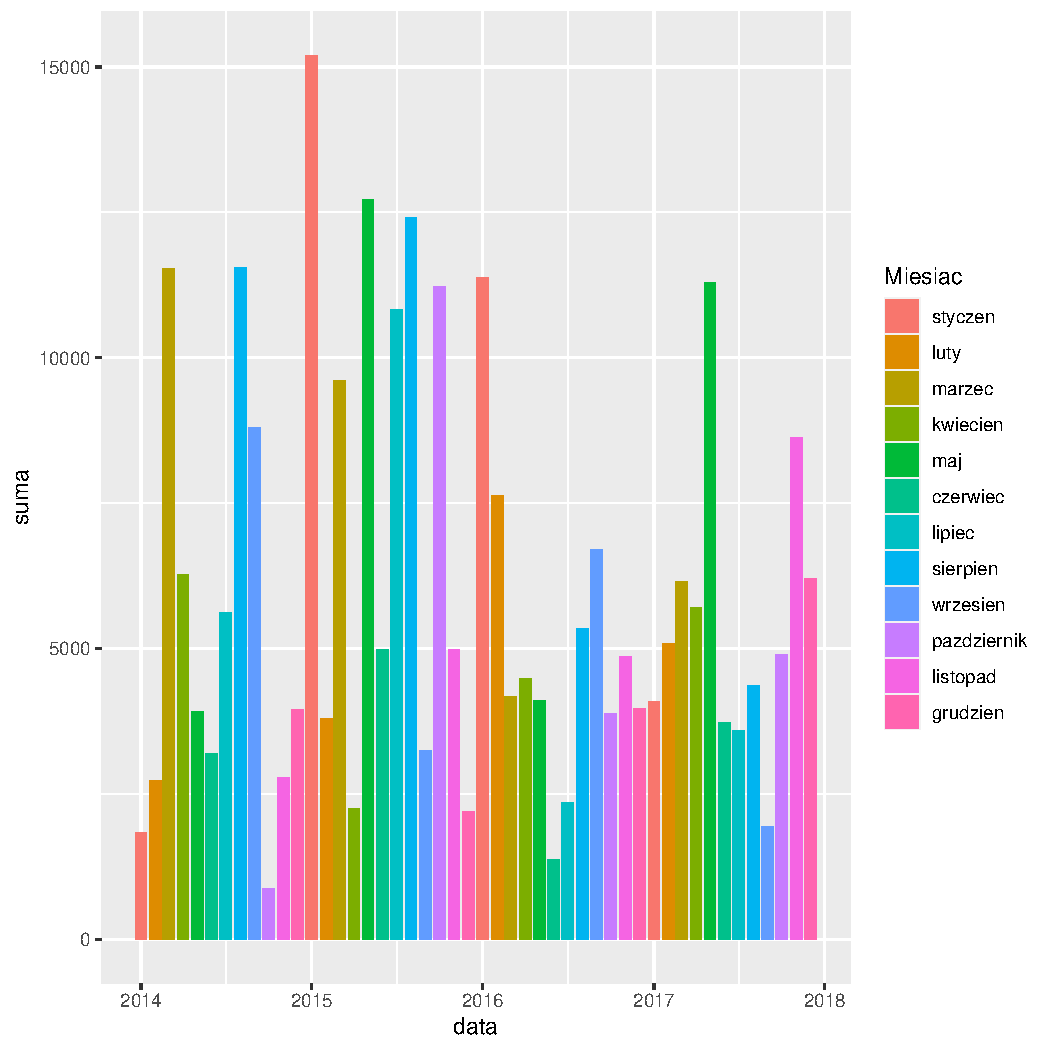
\includegraphics[width=\maxwidth]{figure/unnamed-chunk-6-1} 
\end{knitrout}

\subsection{Analiza przychodów z usług warsztatu}

Chcielibyśmy sprawdzić, jak wyglądają miesięczne przychody (lub straty) wynikające z prowadzenia warsztatu. Przez przychód za pojedyńczą usługę uważamy różnicę ceny, którą zapłacił klient i kwoty zapłaconej za części.

\begin{knitrout}
\definecolor{shadecolor}{rgb}{0.969, 0.969, 0.969}\color{fgcolor}
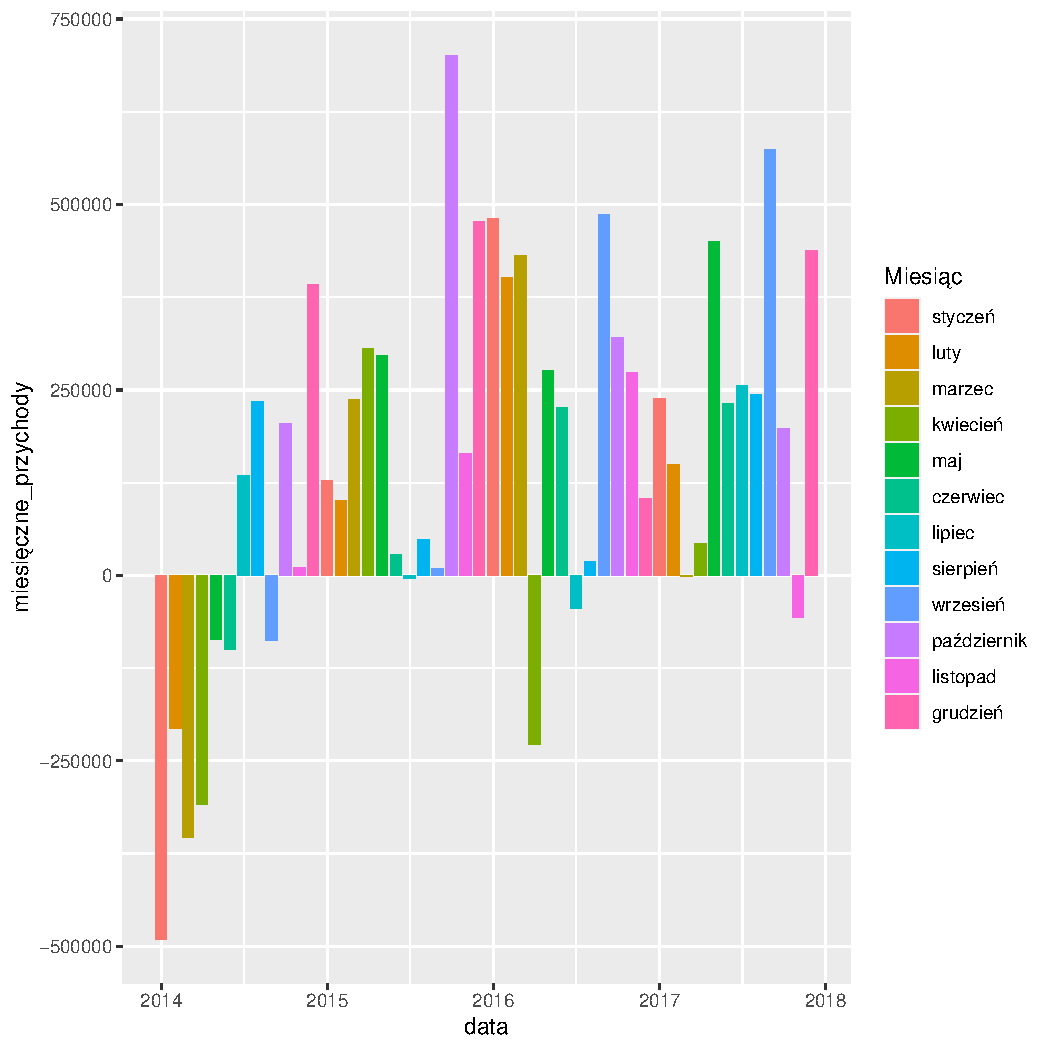
\includegraphics[width=\maxwidth]{figure/unnamed-chunk-7-1} 
\end{knitrout}

{\color{red} tAK JAK WYŻEJ}

\begin{knitrout}
\definecolor{shadecolor}{rgb}{0.969, 0.969, 0.969}\color{fgcolor}
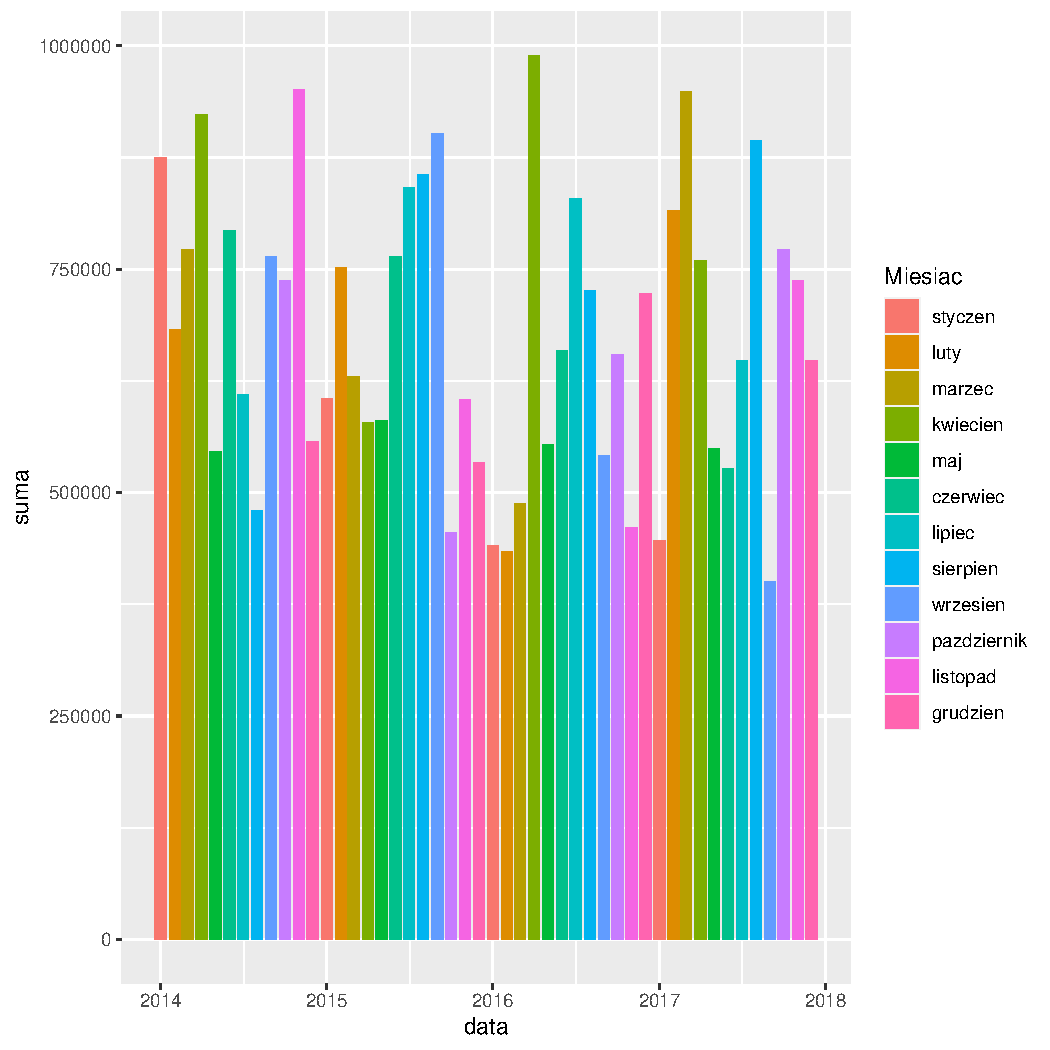
\includegraphics[width=\maxwidth]{figure/unnamed-chunk-8-1} 
\end{knitrout}

{\color{red} SAME ZYSKI, WŁASNYCH NIE LICZYMY}

\subsection{Koszty wypłat dla pracowników}

{\color{red} NA RAZIE NIE MAM}

\subsection{Samochody wpływy}

{\color{red} MOŻE BYĆ TRUDNE BO RATY}

\subsection{Razem na miesiąc}

{\color{red} JAK TO WYZEJ SIĘ UDA}


\section{Kim są najlepszy mechanik i sprzedawca w warsztacie?}

Przez czas działania warsztatu „Pimp My Wheels” osoba zarządzająca warsztatem nie była skłonna do dawania podwyżek, jednak postanowiła zlecić informatykowi by przeanalizował bazę danych i znalazł pracowników, którzy zasługują na większe wynagrodzenie. \\

Warsztatowi zależy na tym by sprzedawca zarobił dla firmy dużą kwotę (Może to osiągnąć sprzedając bardzo dużo pojazdów albo sprzedając wartościowe pojazdy), ale także by był charyzmatyczny i był w stanie przekonać wiele osób do zakupu. Rozważone wobec tego zostanie to który obecnie pracujący sprzedawca przekonał klientów do kupna największej liczby pojazdów, a który odpowiada za najwięcej środków pochodzących ze sprzedaży. \\


Tabela, w której dane o sprzedawcach  pracujących w dowolnym momencie w warsztacie wygląda następująco:



Jeżeli pracownik odszedł z warsztatu, to nielogicznym jest, by rozważać danie mu podwyżki.

Po usunięciu pracowników, którzy już nie pracują otrzymujemy taką tabelę:

\begin{knitrout}
\definecolor{shadecolor}{rgb}{0.969, 0.969, 0.969}\color{fgcolor}\begin{kframe}
\begin{verbatim}
##        sprzedawca     suma ile_sprzedanych płaca id_pracownika status
## 1 Dorota Drewniak 19783751             360  53.8             3      1
\end{verbatim}
\end{kframe}
\end{knitrout}

MUSZE DODAC TEKST JAKBY BYLY DWIE OSOBY \\

Obecnie tylko jedna osoba pracuje w firmie na tym stanowisku i jest to Dorota Drewniak. Ta osoba zarobiła dla firmy 19783750.86 zł na sprzedaży pojazdów, co stanowi 87.81\% średniej kwoty zarobionej przez pracownika dla warsztatu przez cały okres działania warsztatu. W porównaniu, zarabiana przez tego pracownika kwota za godzinę pracy (53.80 zł) stanowi 94.97 \% średniej płacy sprzedawcy (56.65 zł). Różnica procentowa wynosi 7.16\% na korzyść pracownika, jednak biorąc pod uwagę, że to jedyna osoba pracująca obecnie jako sprzedawca w warsztacie i była porównywana z byłymi pracownikami, można spróbować zaoferować podniesienie stawki, by pozytywnie wpłynąć na jej motywację. \\

Ten sprzedawca namówił klientów do kupna 360 pojazdów, co stanowi 93.26\% ilości sprzedanych kiedykolwiek pojazdów dzielonej przez liczbę kiedykolwiek zatrudnionych pracowników. Podobnie jak wcześniej, możemy porównać zarobki, tylko teraz biorąc pod uwagę ilość sprzedaży. Róznica między stosunkiem zarobków do średniej płacy i sprzedanych przez obecnego sprzedawcę samochodów do średniej liczby przypadającej na sprzedawcę  wynosi 1.70\%. Gdyby jedynie brać pod uwagę ilość sprzedaży przy analizie to można zauważyć, że różnica jest na korzyść pracownika. Drobna odwyżka może jednak okazać się dla niej dobrym motywatorem. 

\begin{knitrout}
\definecolor{shadecolor}{rgb}{0.969, 0.969, 0.969}\color{fgcolor}\begin{kframe}
\begin{verbatim}
##         mechanik   suma ile_napraw płaca id_pracownika status
## 1 Wojciech Raźny  85264        214  59.1             6      0
## 2  Dariusz Kuraś 120170        253  45.4             7      1
## 3  Józef Stępień 122724        207  53.0             4      1
\end{verbatim}
\end{kframe}
\end{knitrout}


Tutaj również należy usunąć z tabeli mechaników, którzy już nie pracują w warsztacie. \\

Pozostali następujący pracownicy:

\begin{knitrout}
\definecolor{shadecolor}{rgb}{0.969, 0.969, 0.969}\color{fgcolor}\begin{kframe}
\begin{verbatim}
##        mechanik   suma ile_napraw płaca id_pracownika status
## 1 Dariusz Kuraś 120170        253  45.4             7      1
## 2 Józef Stępień 122724        207  53.0             4      1
\end{verbatim}
\end{kframe}
\end{knitrout}

MUSZE DODAC TEKST JAKBY BYLY DWIE OSOBY \\

Mechanik, który wykonał w firmie naprawy, za które klienci (po odliczeniu kosztu części) zapłacili najwięcej toJózef Stępieńi jest to kwota 122724.00 zł, co stanowi 112.19\% średniego zysku z napraw na mechanika. Pracownik zarabia kwotę 53.00 zł za godzinę pracy, co stanowi 100.95 \% średniej płacy mechanika (52.50 zł). Różnica między tymi wartościami to 11.24\%, wobec czego dobrze by było, gdyby firma zauważyła świetne wyniki tego pracownika i jego pozytywny wpływ na finanse warsztatu. \\

Pracownik, który dokonał największej liczby napraw to Dariusz Kuraś. Ta osoba naprawiła aż 253 pojazdów, co stanowi 112.95\% średniej ilości napraw na mechanika. Jej zarobki wynoszą 45.40 zł na godzinę, co stanowi 86.48 \% średniej płacy mechanika (52.50 zł). Różnica między tymi dwoma wartościami wynosi 26.47\%, więc podwyżka wydaje się rozsądnym rozwiązaniem, aby okazać mechanikowi, że warsztat go docenia.



\end{document}
